\documentclass[aspectratio=169]{beamer}

% Theme selection
\usetheme{Madrid}
\usecolortheme{default}

% Packages
\usepackage[utf8]{inputenc}
\usepackage[T1]{fontenc}
\usepackage{amsmath,amssymb}
\usepackage{tikz}
\usetikzlibrary{arrows.meta,positioning}
\usepackage{pgfplots}
\pgfplotsset{compat=1.18}

% Metadata
\title[\textbf{Autonomous Scientific Overleaf}]{\textbf{Autonomous AI Agent Workflows in Scientific Publishing}}
\subtitle{Containerized Compilation and Headless Overleaf Automation}
\author[Antigravity Team]{Antigravity Agentic Systems Research}
\institute[DeepMind / Community]{Research \& Development Engineering}
\date{\today}

\begin{document}

% Slide 1: Title
\begin{frame}
  \titlepage
\end{frame}

% Slide 2: Overview & Motivation
\begin{frame}{Motivation: Decoupling Reasoning from Typesetting}
  \begin{columns}
    \begin{column}{0.5\textwidth}
      \textbf{Core Challenges in Agent Publishing:}
      \begin{itemize}
        \item Complex mathematical formatting ($\mathbb{R}^n$, $\det(\mathbf{A})$).
        \item Host environment contamination with multi-GB TeX trees.
        \item Multi-architecture cross-platform execution.
      \end{itemize}
    \end{column}
    \begin{column}{0.5\textwidth}
      \textbf{The Containerized Solution:}
      \begin{block}{Headless Overleaf Stack}
        \begin{itemize}
          \item Programmatic REST API endpoints.
          \item Zero browser launchpad setup.
          \item Sub-second incremental caching.
        \end{itemize}
      \end{block}
    \end{column}
  \end{columns}
\end{frame}

% Slide 3: TikZ Architecture in Beamer
\begin{frame}{Architecture: Programmatic Feedback Loop}
  \centering
  \resizebox{0.88\textwidth}{!}{%
  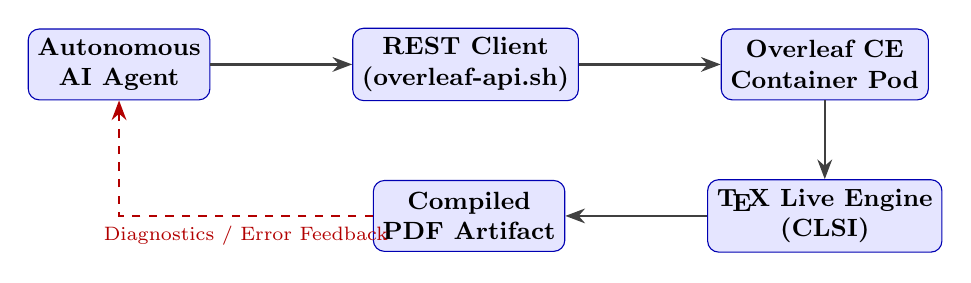
\begin{tikzpicture}[
      node distance=1.8cm,
      box/.style={draw=blue!70!black, fill=blue!10, rounded corners=4pt, align=center, font=\small\bfseries, minimum height=0.9cm, minimum width=2.2cm},
      arrow/.style={-{Stealth[length=2.5mm]}, thick, darkgray},
      feedback/.style={-{Stealth[length=2.5mm]}, thick, dashed, red!70!black}
  ]
      \node[box] (agent) {Autonomous\\AI Agent};
      \node[box, right=of agent] (api) {REST Client\\(overleaf-api.sh)};
      \node[box, right=of api] (server) {Overleaf CE\\Container Pod};
      \node[box, below=1cm of server] (clsi) {\TeX\ Live Engine\\(CLSI)};
      \node[box, left=of clsi] (pdf) {Compiled\\PDF Artifact};

      \draw[arrow] (agent) -- (api);
      \draw[arrow] (api) -- (server);
      \draw[arrow] (server) -- (clsi);
      \draw[arrow] (clsi) -- (pdf);
      \draw[feedback] (pdf) -| (agent) node[pos=0.25, below, font=\scriptsize] {Diagnostics / Error Feedback};
  \end{tikzpicture}
  }
\end{frame}

% Slide 4: Empirical Benchmark Plot
\begin{frame}{Performance: Incremental vs. Cold Compilation}
  \centering
  \resizebox{0.78\textwidth}{!}{%
  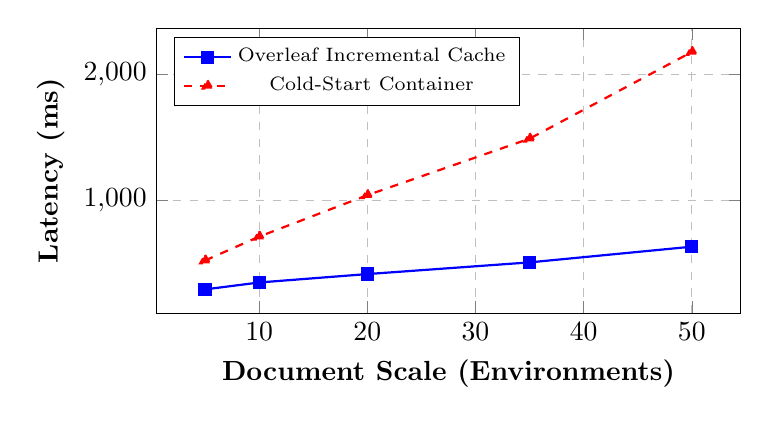
\begin{tikzpicture}
  \begin{axis}[
      width=9cm,
      height=5.2cm,
      xlabel={\textbf{Document Scale (Environments)}},
      ylabel={\textbf{Latency (ms)}},
      grid=both,
      grid style=dashed,
      legend pos=north west,
      legend style={font=\scriptsize}
  ]
  \addplot[color=blue, mark=square*, thick] coordinates {
      (5, 290) (10, 345) (20, 412) (35, 505) (50, 630)
  };
  \addlegendentry{Overleaf Incremental Cache}

  \addplot[color=red, mark=triangle*, thick, dashed] coordinates {
      (5, 520) (10, 710) (20, 1040) (35, 1490) (50, 2180)
  };
  \addlegendentry{Cold-Start Container}
  \end{axis}
  \end{tikzpicture}
  }
\end{frame}

% Slide 5: Summary
\begin{frame}{Conclusion}
  \begin{exampleblock}{Key Takeaways}
    \begin{enumerate}
      \item Full \textbf{Beamer presentation} support pre-baked in the container.
      \item Built-in support for \textbf{TikZ} graphics and \textbf{PGFPlots} charts.
      \item Dual access: Direct unauthenticated PDF links or full collaborative IDE.
    \end{enumerate}
  \end{exampleblock}
  \vspace{0.5cm}
  \centering
  \textbf{Ready for Autonomous Agent Workflows!}
\end{frame}

\end{document}
